\section{Introduction}

This guide is intended to get you started running Linux (Ubuntu port provided by \href{http://www.linaro.org}{Linaro} and developed by krtkl) on snickerdoodle. This guide uses programs and utilities on a Linux host computer (or virtual machine) to install a complete Linux system that snickerdoodle will boot from a microSD card. A Linux (krtkl recommends the latest \href{http://www.ubuntu.com/download/desktop/}{LTS release from Ubuntu}) system with the ability to mount a microSD card (UHS Speed Class 3 recommended) is required to install the Linux system.

\begin{marginfigure}
	\centering
	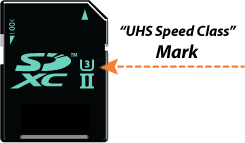
\includegraphics{images/card-marks-en.png}
	\caption[SD Card UHS Speed Class Marking adapted from \url{https://www.sdcard.org/consumers/speed/speed_class/}]{SD Card UHS Speed Class Marking (adapted from \url{https://www.sdcard.org/consumers/speed/speed_class/})}
\end{marginfigure}

\section{Formatting SD Card}

\subsection{Locating SD Card on System}
\label{sub:locatesd}

The \texttt{mount} command can be used to locate the SD card device, once it has been connected to the host computer. In the example below, an SD card has been connected on \texttt{/dev/sdb1} and mounted at \texttt{/media/user/UNTITLED}. \\

\begin{lstlisting}[style=text]
$ mount
/dev/sda1 on / type ext4 (rw,errors=remount-ro)
proc on /proc type proc (rw,noexec,nosuid,nodev)
sysfs on /sys type sysfs (rw,noexec,nosuid,nodev)
none on /sys/fs/cgroup type tmpfs (rw)
none on /sys/fs/fuse/connections type fusectl (rw)
...
(*@\bfseries\color{red}{/dev/sdb1}@*) on (*@\bfseries\color{red}{/media/user/UNTITLED}@*) type vfat (rw,nosuid,nodev,uid=1000,gid=1000,shortname=mixed,dmask=0077, utf8=1,showexec,flush,uhelper=udisks2)
\end{lstlisting}

\subsection{Partitioning the SD Card (\texttt{fdisk})}
Before partitioning the SD card, any partitions that have been mounted on the system must be unmounted. This can be done using the \texttt{umount} command. \\

\begin{lstlisting}
$ umount /dev/sdb1
\end{lstlisting}

~\\
\noindent
Once the SD card has been located, we can partition it for the Linux system (\textit{BOOT} partition) and root filesystem (\textit{ROOTFS} partition) using \texttt{fdisk}\sidenote{Additional information on \texttt{fdisk} can be found at: \url{http://tldp.org/HOWTO/Partition/fdisk_partitioning.html}}. \texttt{fdisk} must be run with root permissions (\texttt{sudo}) using the disk parent as the argument (do not use the partition number in the argument).\\ 

\margincautionnote{Do NOT include any partition number (in the example case '1') when running \texttt{fdisk} on the SD card. '\texttt{/dev/sdb}' NOT '\texttt{/dev/sdb1}'}

\begin{lstlisting}[language=bash]
$ sudo fdisk /dev/sdb
\end{lstlisting}

~\\
\noindent
From within the \texttt{fdisk} interface, we can view the partition table at any time using the 'p' command. In this example, an 8GB SD card with a single FAT32 partition is being used and will be re-partitioned for snickerdoodle. \\

\begin{lstlisting}[style=text]
Command (m for help): (*@\bfseries\color{red}{p}@*)

Disk /dev/sdb: 7969 MB, 7969177600 bytes
255 heads, 63 sectors/track, 968 cylinders, total 15564800 sectors
Units = sectors of 1 * 512 = 512 bytes
Sector size (logical/physical): 512 bytes / 512 bytes
I/O size (minimum/optimal): 512 bytes / 512 bytes
Disk identifier: 0x00000000

   Device Boot      Start         End      Blocks   Id  System
/dev/sdb1            8192    15564799     7778304    b  W95 FAT32
\end{lstlisting}

\subsection{BOOT Partition}
First, a partition must be allocated for the Linux system binaries and files. This includes \texttt{BOOT.bin} (FSBL, bitstream, U-Boot), \texttt{uEnv.txt}, \texttt{devicetree.dtb}, and the Linux kernel \texttt{uImage}. The partition size for these files is recommended to be 128MB in size which translates to an additional 262144, 512 byte sectors. \\

\begin{lstlisting}[style=text]
Command (m for help): (*@\bfseries\color{red}{d}@*)
Selected partition 1

Command (m for help): (*@\bfseries\color{red}{n}@*)
Partition type:
   p   primary (0 primary, 0 extended, 4 free)
   e   extended
Select (default p): (*@\bfseries\color{red}{p}@*)
Partition number (1-4, default 1): (*@\bfseries\color{red}{1}@*)
First sector (2048-15564799, default 2048): (*@\bfseries\color{red}{<RETURN>}@*)
Using default value 2048
Last sector, +sectors or +size{K,M,G} (2048-15564799, default 15564799): (*@\bfseries\color{red}{+262144}@*)
\end{lstlisting}


~\\
\noindent
The default partition type for \texttt{fdisk} is \textbf{Linux} (type ID 83). The \textit{BOOT} partition needs to be formatted as \textbf{FAT32} (type ID 'C'). To do this, the 't' command is used: \\

\begin{lstlisting}[style=text]
Command (m for help): (*@\bfseries\color{red}{t}@*)
Partition number (1-4): (*@\bfseries\color{red}{1}@*)
Hex code (type L to list codes): (*@\bfseries\color{red}{c}@*)
Changed system type of partition 1 to c (W95 FAT32 (LBA))
\end{lstlisting}

\subsection{ROOTFS Partition}
Second, a partition for the root filesystem must be created. This partition will be formatted as a \textbf{Linux} type using type ID 83. This is the default partition type. \\
\begin{lstlisting}[style=text]
Command (m for help): (*@\bfseries\color{red}{n}@*)
Partition type:
   p   primary (1 primary, 0 extended, 3 free)
   e   extended
Select (default p): (*@\bfseries\color{red}{p}@*)
Partition number (1-4, default 2): (*@\bfseries\color{red}{<RETURN>}@*)
Using default value 2
First sector (264193-15564799, default 264193): (*@\bfseries\color{red}{<RETURN>}@*)
Using default value 264193
Last sector, +sectors or +size{K,M,G} (264193-15564799, default 15564799): (*@\bfseries\color{red}{<RETURN>}@*)
Using default value 15564799
\end{lstlisting}

\margininfonote{Always check the partition table before attempting to write it to the disk, using the 'p' command.}

~\\
\noindent
Before writing the partition table, you should verify the partition layout by printing it with the 'p' command. In this example, an 8GB SD card has been partitioned with a 128MB FAT32 \textit{BOOT} partition and the rest allocated for a Linux \textit{ROOTFS} partition. \\

\begin{lstlisting}[style=text]
Command (m for help): (*@\bfseries\color{red}{p}@*)

Disk /dev/sdb: 7969 MB, 7969177600 bytes
255 heads, 63 sectors/track, 968 cylinders, total 15564800 sectors
Units = sectors of 1 * 512 = 512 bytes
Sector size (logical/physical): 512 bytes / 512 bytes
I/O size (minimum/optimal): 512 bytes / 512 bytes
Disk identifier: 0x00000000

   Device Boot      Start         End      Blocks   Id  System
/dev/sdb1            2048      264192      131072+   c  W95 FAT32 (LBA)
/dev/sdb2          264193    15564799     7650303+  83  Linux
\end{lstlisting}

~\\
\noindent
Once the partition table has been verified, the 'w' command can be used to write the table to the disk: \\
\begin{lstlisting}[style=text]
Command (m for help): (*@\bfseries\color{red}{w}@*)
The partition table has been altered!

Calling ioctl() to re-read partition table.
Syncing disks.
\end{lstlisting}

\section{Formatting Partitions (\texttt{mkfs}/\texttt{mke2fs})}
With a partitioned SD card, the partitions need to be formatted with the necessary filesystem type. For the \textit{BOOT} partition, the filesystem type is \textbf{VFAT}. Formatting the \textit{BOOT} partition can be done using the \texttt{mkfs.vfat}\sidenote{Additional information on \texttt{mkfs/mke2fs} and it's front end tools can be found at: \url{http://www.tldp.org/HOWTO/Partition/formatting.html}}. To format a FAT32 filesystem on \texttt{/dev/sdb1} with a 'BOOT' disk label, the following command can be used: \\

\begin{lstlisting}
$ sudo mkfs.vfat -n BOOT /dev/sdb1
\end{lstlisting}

~\\
\noindent
The format for the \textit{ROOTFS} partition can be done with \texttt{mke2fs} which will format a Linux partition with an ext2/ext3/ext4 filesystem. To format an ext4 filesystem on \texttt{/dev/sdb2} with a block size of 1k (1024) and a 'ROOTFS' disk label, the following command can be used: \\

\margincautionnote{When formatting disk partitions, make sure the disk partitions are NOT mounted.}

\begin{lstlisting}
$ mke2fs -b 1024 -t ext4 -L ROOTFS /dev/sdb2
\end{lstlisting}


~\\
\noindent
If the formatting is successful, the following output will be written to the console (writing superblocks and filesystem accounting information can take some time depending on the size and speed of the SD card): \\

\begin{lstlisting}[style=text]
mke2fs 1.42.9 (4-Feb-2014)
Filesystem label=ROOTFS
OS type: Linux
Block size=4096 (log=0)
Fragment size=4096 (log=0)
Stride=0 blocks, Stripe width=0 blocks
478208 inodes, 7650300 blocks
382515 blocks (5.00%) reserved for the super user
First data block=1
Maximum filesystem blocks=74973184
934 block groups
8192 blocks per group, 8192 fragments per group
512 inodes per group
Superblock backups stored on blocks: 
	8193, 24577, 40961, 57345, 73729, 204801, 221185, 401409, 663553, 
	1024001, 1990657, 2809857, 5120001, 5971969

Allocating group tables: done                            
Writing inode tables: done                            
Creating journal (32768 blocks): done
Writing superblocks and filesystem accounting information: done   
\end{lstlisting}


~\\
\noindent
After the partitions have been properly formatted, the SD card must be ejected and re-connected before moving the Linux boot components and root filesystem contents to the disk. \\

\begin{lstlisting}
$ eject /dev/sdb
\end{lstlisting}


\section{Sources}

\subsection{BOOT Partition Components}

The latest \textit{BOOT} partition Linux components for Snickerdoodle and Snickerdoodle Black can be downloaded using \texttt{git}. \\
\begin{lstlisting}[language=bash]
$ git clone https://github.com/krtkl/snickerdoodle-linux-prebuilt.git
\end{lstlisting}

~\\
\noindent
Alternatively, the sources can be downloaded directly from a web browser from the \href{https://github.com/krtkl/snickerdoodle-linux-prebuilt}{krtkl GitHub page} as a \texttt{.ZIP} file.

\begin{figure}[h!]
\centering
	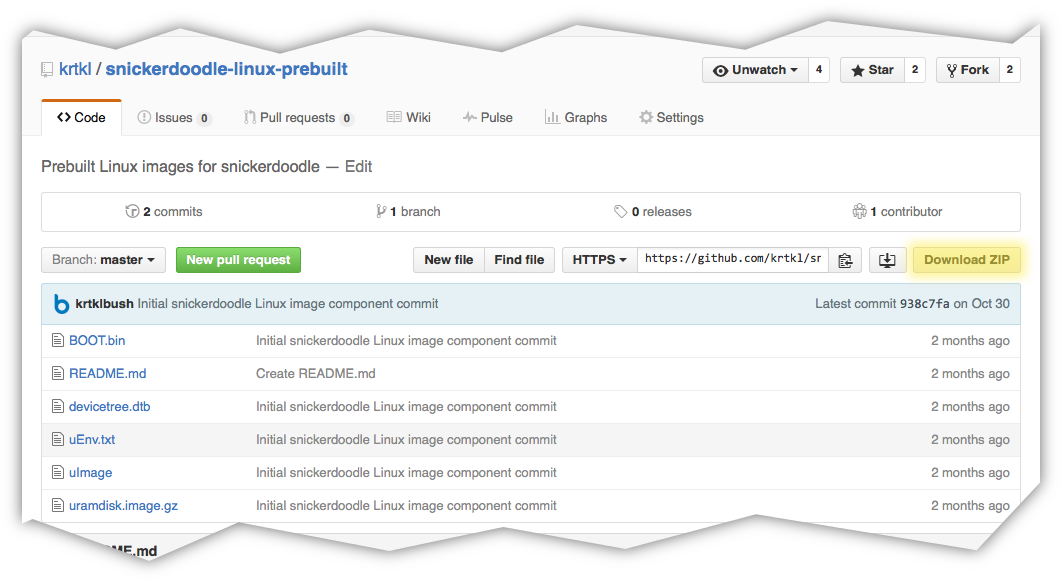
\includegraphics{images/github-prebuilt.png}
	\caption{Download prebuilt Linux components from GitHub}
	\label{fig:githubprebuilt}
\end{figure}


\subsection{Copy Files to SD Card}
After downloading the SD card components

\noindent
The \textit{BOOT} components can be installed onto the SD card using the \texttt{cp} command, starting with \texttt{BOOT.bin}. In this example, the files are copied to the \textit{BOOT} partition that has been mounted at \texttt{/media/user/BOOT}. As stated above, the \texttt{mount} command can be used to \hyperref[sub:locatesd]{locate the mount point of the SD card partitions}. \\

\begin{lstlisting}
$ cd snickerdoodle-linux-prebuilt/snickerdoodle
$ cd boot_images
$ cp BOOT.bin /media/$USER/BOOT
$ cp uEnv.txt /media/$USER/BOOT
$ cp devicetree.dtb /media/$USER/BOOT
$ cp uImage /media/$USER/BOOT
\end{lstlisting}

~\\
\noindent
After copying the \textit{BOOT} components, the \texttt{sync} command should be used to make sure the system buffers have been flushed and the process of writing the files to the SD card is complete. \\

\begin{lstlisting}
$ sync
\end{lstlisting}

\subsection{ROOTFS Sources}

The root filesystem can be extracted directly into the \textit{ROOTFS} partition using the '-C' argument when extracting the archive contents. An Ubuntu 14.04 filesystem can be downloaded from \url{http://krtkl.com/downloads/}. In this example, the \textit{ROOTFS} partition is mounted at \texttt{/media/user/ROOTFS}, which should be checked before attempting to extract the root filesystem. The root filesystem contains a lot of large packages (ROS, python, etc.) and may take several minutes to complete the process of writing to the SD card. \\

\begin{lstlisting}
$ tar -C /media/$USER/ROOTFS -xvzf snickerdoodle-ubuntu-14.04.tar.gz
\end{lstlisting}


~\\
\noindent
After extracting the root filesystem to the SD card, use the \texttt{sync} command to flush the system buffers and ensure the write process is complete. Additionally, making sure to unmount the SD card partitions before ejecting will make certain that any lingering write processes have completed before the SD card is removed. \\


\begin{lstlisting}
$ sync
$ umount /dev/sdb1
$ umount /dev/sdb2
$ eject /dev/sdb
\end{lstlisting}


~\\
\noindent
Now that the microSD card has been partitioned, formatted and populated with the Linux files, it is ready to be installed onto snickerdoodle and booted. Install the microSD card into the card cage (J6) and connect power on either the micro USB connector (J1) or the power pins on J2. The familiar Ubuntu boot console should start and you will have access to a terminal to begin configuration and development of snickerdoodle. 

\begin{figure}
	\centering
	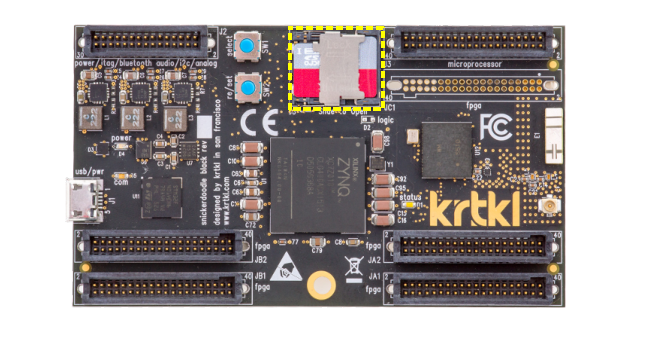
\includegraphics{images/SD_microSD.pdf}
	\caption{snickerdoodle SD Card Connector with Installed microSD Card}
\end{figure}


\begin{fullwidth}
\begin{lstlisting}[%
  backgroundcolor=\color{black},
  basicstyle={\small\ttfamily\color{green}}
  ]
Welcome to Ubuntu 14.04 (GNU/Linux 3.14.0-xilinx-dirty armv7l)

 * Documentation:  http://www.ubuntu.com
root@snickerdoodle:~/workspace# python hello_world.py 
Congratulations! You've run your first python script on snickerdoodle!
\end{lstlisting}
\end{fullwidth}

